\everymath{\displaystyle}
%\documentclass[pdftex,a4paper]{article}
\documentclass[a4paper]{article}
%%classes: article, report, book, proc, amsproc

%%%%%%%%%%%%%%%%%%%%%%%%
%% Misc
% para acertar os acentos
\usepackage[brazilian]{babel} 
%\usepackage[portuguese]{babel} 
% \usepackage[english]{babel}
% \usepackage[T1]{fontenc}
% \usepackage[latin1]{inputenc}
\usepackage[utf8]{inputenc}
\usepackage{indentfirst}
\usepackage{fullpage}
% \usepackage{graphicx} %See PDF section
\usepackage{multicol}
\setlength{\columnseprule}{0.5pt}
\setlength{\columnsep}{20pt}
%%%%%%%%%%%%%%%%%%%%%%%%
%%%%%%%%%%%%%%%%%%%%%%%%
%% PDF support

\usepackage[pdftex]{color,graphicx}
% %% Hyper-refs
\usepackage[pdftex]{hyperref} % for printing
% \usepackage[pdftex,bookmarks,colorlinks]{hyperref} % for screen

%% \newif\ifPDF
%% \ifx\pdfoutput\undefined\PDFfalse
%% \else\ifnum\pdfoutput > 0\PDFtrue
%%      \else\PDFfalse
%%      \fi
%% \fi

%% \ifPDF
%%   \usepackage[T1]{fontenc}
%%   \usepackage{aeguill}
%%   \usepackage[pdftex]{graphicx,color}
%%   \usepackage[pdftex]{hyperref}
%% \else
%%   \usepackage[T1]{fontenc}
%%   \usepackage[dvips]{graphicx}
%%   \usepackage[dvips]{hyperref}
%% \fi

%%%%%%%%%%%%%%%%%%%%%%%%


%%%%%%%%%%%%%%%%%%%%%%%%
%% Math
\usepackage{amsmath,amsfonts,amssymb}
% para usar R de Real do jeito que o povo gosta
\usepackage{amsfonts} % \mathbb
% para usar as letras frescas como L de Espaco das Transf Lineares
% \usepackage{mathrsfs} % \mathscr

% Oferecer seno e tangente em pt, com os comandos usuais.
\providecommand{\sin}{} \renewcommand{\sin}{\hspace{2pt}\mathrm{sen}}
\providecommand{\tan}{} \renewcommand{\tan}{\hspace{2pt}\mathrm{tg}}

% dt of integrals = \ud t
\newcommand{\ud}{\mathrm{\ d}}
%%%%%%%%%%%%%%%%%%%%%%%%



\begin{document}

%%%%%%%%%%%%%%%%%%%%%%%%
%% Título e cabeçalho
%\noindent\parbox[c]{.15\textwidth}{\includegraphics[width=.15\textwidth]{logo}}\hfill
\parbox[c]{.825\textwidth}{\raggedright%
  \sffamily {\LARGE

Equações Diferenciais: Notas de Aula

Modelagem matemática com EDOs de primeira ordem

\par\bigskip}
{Prof: Felipe Figueiredo\par}
{\url{http://sites.google.com/site/proffelipefigueiredo}\par}
}

Versão: \verb|20150905|

%%%%%%%%%%%%%%%%%%%%%%%%


%%%%%%%%%%%%%%%%%%%%%%%%
\section{Objetivos de aprendizagem}

Ao final desta aula o aluno deve saber \ldots


\section{Pré-requitos da aula}

\begin{itemize}
\item 
\item 
\end{itemize}

\section{Conteúdo}

O aluno deve consultar o livro texto na seção X.Y para se aprofundar
no conteúdo desta aula.


\subsection{Resistência do ar}

Como funciona um pára-quedas?

Um corpo em queda livre tem sua velocidade acelerada pela força da
gravidade. Assim, a força que atua no corpo, para baixo é $F_g=mg$, onde
$m$ é a massa e $g$ é a aceleração da gravidade, que assumiremos
constante por simplicidade.

O pára-quedas tem a função de diminuir ou cancelar essa aceleração,
atuando na direção oposta (a força atua para cima). Ele cria uma
enorme resistência do ar que é {\rm proporcional} à velocidade
atual. Assim, a força gerada pelo pára-quedas pode ser escrita como
$F_p=\alpha v$. Isso implica que, quanto maior for a velocidade, maior
será também a resistência do ar (diretamente proporcionais).

A resultante dessas duas forças é a diferença entre ambas, isto é
$F=F_g-F_p$. Pela segunda lei de Newton essa força resultante é
$F=m v'$, onde $v'$ é a aceleração. Juntando tudo em uma única
equação, temos:

\begin{displaymath}
  m v' = mg - \alpha v
\end{displaymath}

Simplificando, isto é, dividindo por $m$, temos:

\begin{displaymath}
  v' = g - \frac{\alpha}{m} v
\end{displaymath}

Podemos colocar o coeficiente de $v$ em evidência, no lado direito da
igualdade, dividindo ambos os termos por ele:

\begin{displaymath}
  v' = g - \frac{\alpha}{m} v = - \frac{\alpha}{m} v +g
\end{displaymath}

\begin{displaymath}
  v' =  -\frac{\alpha}{m} ( v - \frac{mg}{\alpha})
\end{displaymath}

Agora, com o coeficiente de $v$ do lado direito em evidência, fica um
pouco mais fácil para separar as variáveis e resolver a equação.

{\bf Exemplo:}

Josefina salta de um avião e abre o pára-quedas imediatamente. Sua
velocidade inicial é $v_0=0$. Jô pesa $50kg$ e digamos que o
coeficiente de arrasto do ar nesse local é $\alpha = 50$. Assumindo
que a gravidade é $g=10\frac{m}{s^2}$, qual será a velocidade de Jô
após os primeiros $2s$ de pura adrenalina?

{\bf Resolução:}

Substituindo as informações do enunciado temos:

\begin{displaymath}
  v' =  -\frac{50}{50} ( v - \frac{50 \times 10}{50}) = - (v - 10)
\end{displaymath}

Agora já podemos resolver o:

PVI pára-quedas: $\left\{
    \begin{array}{l}
      v' = - (v - 10)
      \\
      \\
      v(0)=0
    \end{array}
  \right.$

A família de soluções da EDO é $v(t)=K e^{-t}+10$. Substituindo a
velocidade inicial, encontramos o valor de $K$:

$v(0) = K e^0 +10$

$0 = K+10$

$K=-10$

E a solução desse PVI é:

\begin{displaymath}
  v(t) = -10e^{-t}+10
\end{displaymath}

Com essa função, podemos saber a velocidade Jô em qualquer instante de
tempo. Como queremos saber a velocidade depois de $2s$, basta
substituir $t=2$ e encontrar a resposta procurada:

\begin{displaymath}
  v(2)=-10 e^{-2}+10
\end{displaymath}

Como curiosidade, podemos efeturar essa resposta na calculadora e
encontrar um valor numérico aproximado de
$8.6\frac{m}{s} \approx 31\frac{km}{h}$.

\hrulefill

{\bf Desafio 1:} Qual seria a velocidade de Jô depois de $2s$ se ela
não tivesse um pára-quedas? (O que muda no problema?)

\hrulefill

{\bf Desafio 2:} Como a resistência do ar aumenta com a velocidade
causada pela gravidade, em algum momento as duas forças $F_g$ e $F_p$
se igualam e se cancelam, e nesse momento Jô passa a cair com
velocidade constante (força resultante nula $\Rightarrow$ aceleração
nula $\Rightarrow v'=0$). Qual é essa velocidade terminal?

O gráfico abaixo mostra a velocidade terminal:

\begin{center}
  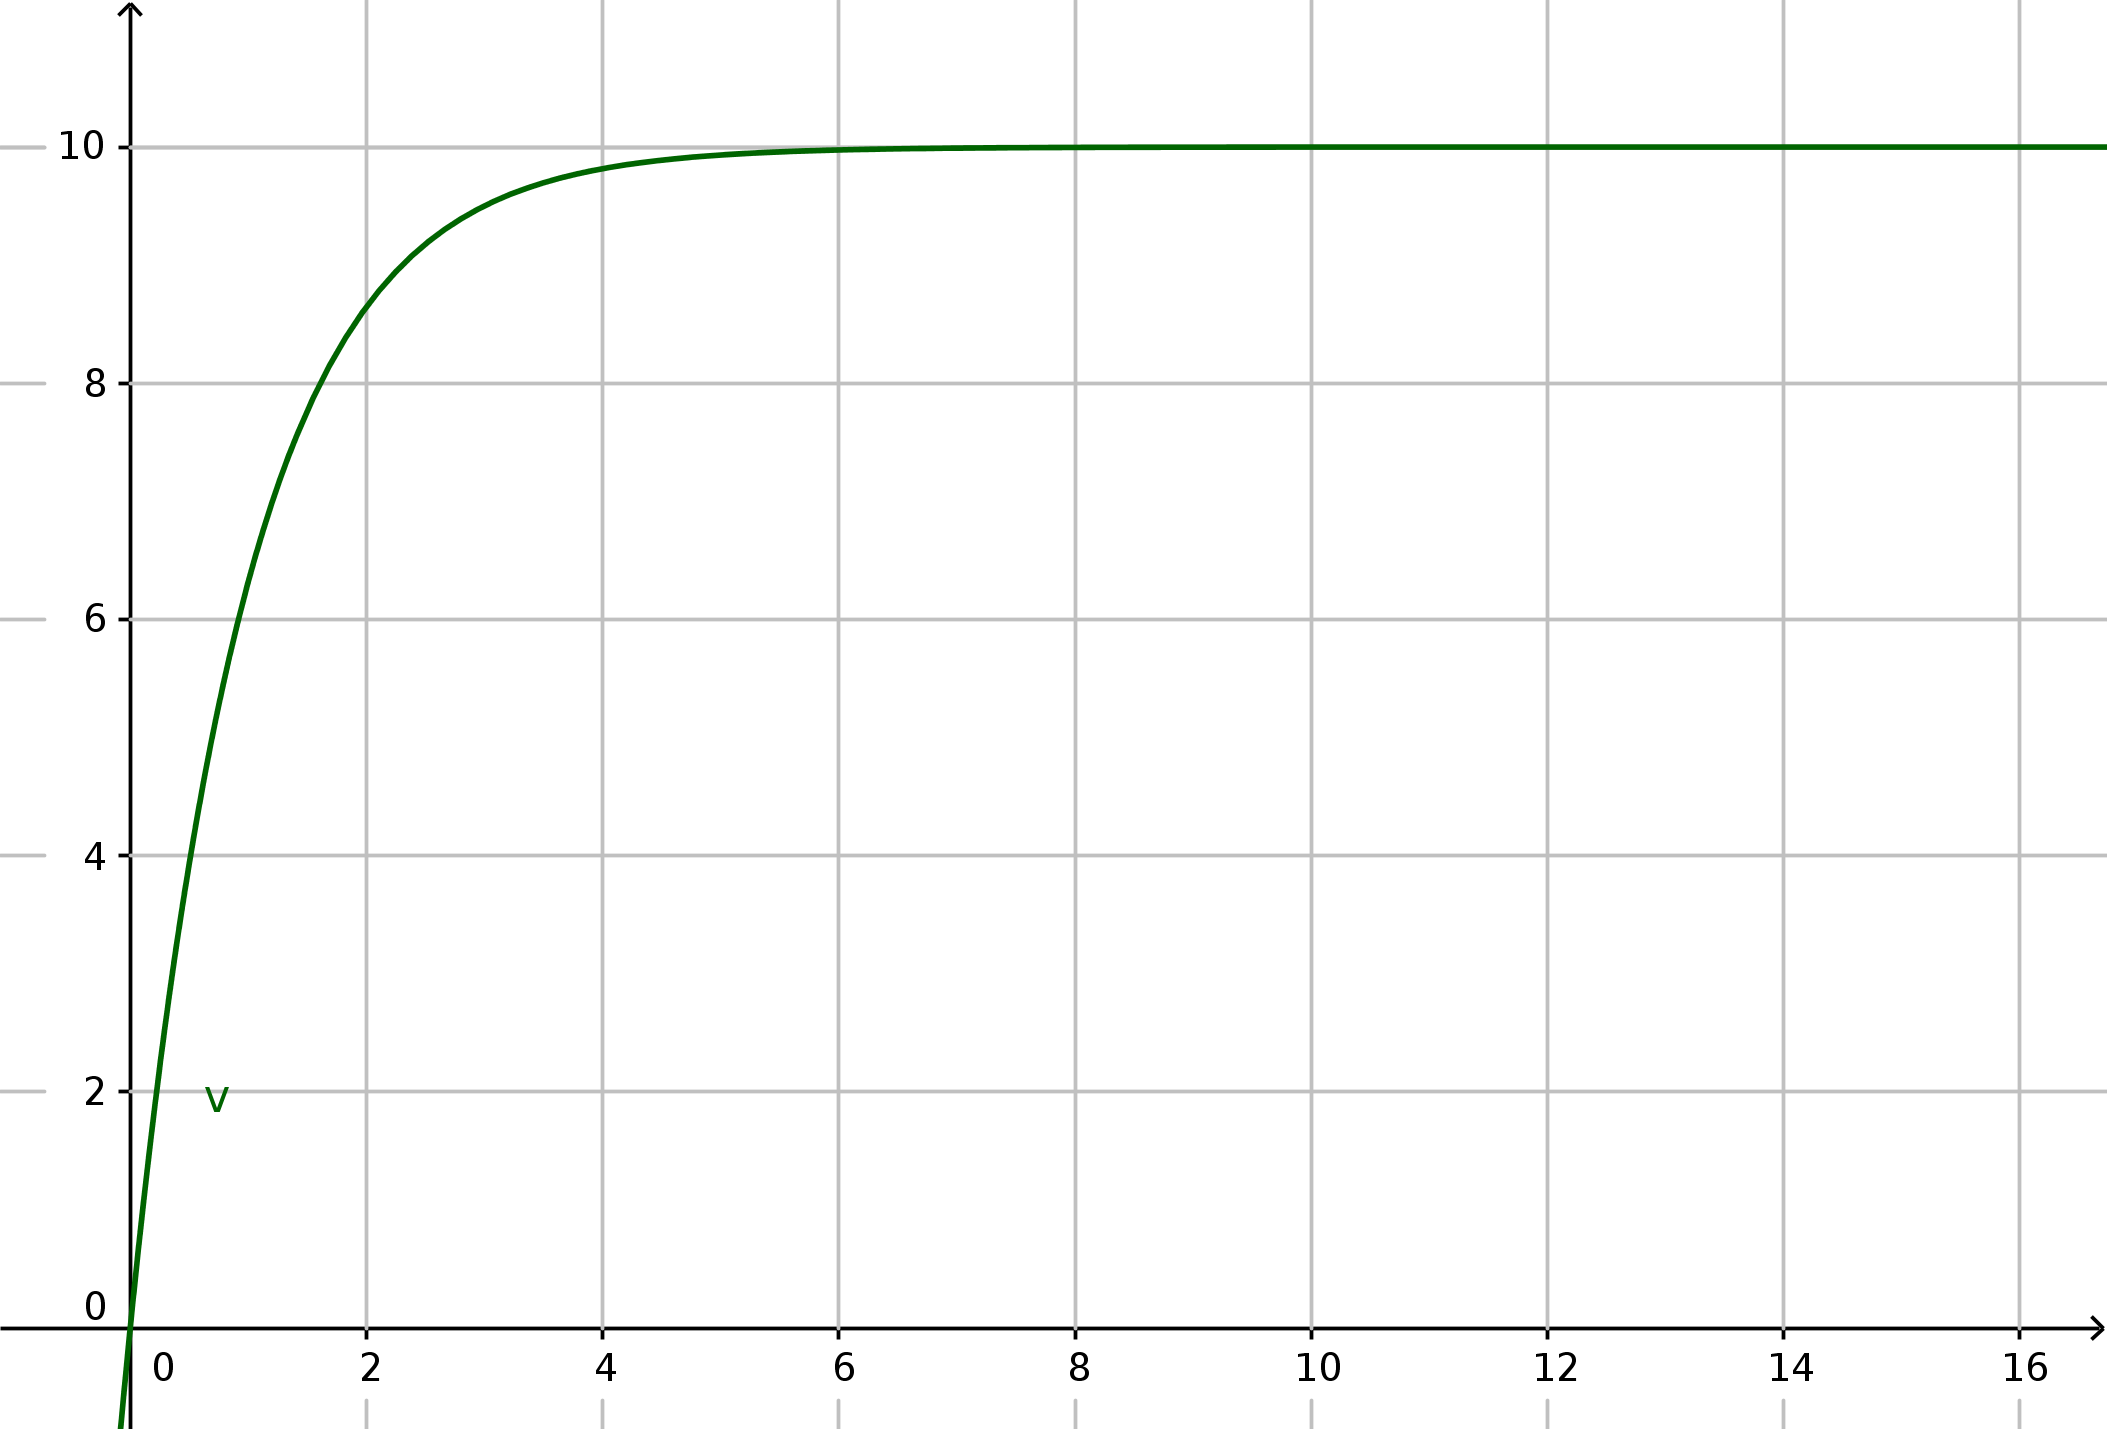
\includegraphics[width=.65\textwidth]{pqd}
\end{center}

\subsection{Lei de Newton do Resfriamento (ou Aquecimento)}

Como exatamente uma tulipa de cerveja esquenta, ou uma xícara de café
esfria com o tempo?

Considere a temperatura $T(t)$ de um objeto, que está em um local onde
a temperatura ambiente $T_a$ é constante.

Em poucas palavras, a {\bf Lei de Newton do Resfriamento} (ou do
aquecimento) diz que ``{\em a temperatura $T$ do corpo tende a se
  igualar com a temperatura $T_a$ do ambiente, a uma taxa proporcional
  à diferença entre ambas, isto é a diferença entre $T$ e $T_a$}''.

Ora, a diferença entre a temperatura do objeto ($T$) e a temperatura
do ambiente ($T_a$) é simplesmente a subtração destes: $T - T_a$. A
variação da temperatura é sua derivada $T'$. Assim, a
proporcionalidade entre essas duas grandezas é dada pela equação

\begin{displaymath}
  T' = -\alpha(T-T_a)
\end{displaymath}

Por que $\alpha$ tem sinal negativo? Observe que conforme o tempo passa, a
diferença entre a temperatura do objeto e a temperatura do ambiente
vai diminuindo. A tendência é que, após um tempo muito grande, essas
temperaturas se igualem. Com isso, a temperatura $T$ do objeto deixa
de variar (ou seja, derivada $T'=0$).

Se você souber o valor da temperatura do ambiente $T_a$, a temperatura
inicial $T(0)$ do objeto e a constante $\alpha$, você pode montar e
resolver um PVI substituindo esses valores na equação acima.

{\bf Exemplos}: Duas pessoas estão em um restaurante, onde a
temperatura ambiente é $T_a=25^o$C. Uma delas pede um café, com
temperatura inicial $90^o$C, e a outra pede um chope com temperatura
inicial $6^o$C. Qual é a função $T(t)$ que determina como a
temperatura de cada um desses objetos varia com o tempo? Considere que
a taxa de transferência nesse local de temperatura é $\alpha=1\%$.

{\bf Resoluções:}

Substituindo os valores $\alpha=\frac{1}{100}$ e $T_a=25$, temos a
equação $T'=-\frac{1}{100}(T-25)$. Para cada uma das temperaturas
iniciais $T(0)$ acima, temos um PVI, conforme abaixo.

Como vimos nas aulas anteriores, a família de soluções da equação
$\frac{\ud T}{\ud t}=-\frac{1}{100}(T-25)$ é: $T(t)=Ke^{-t/100}+25$
(você pode chegar nessa resposta usando separação de variáveis).

Assim, a solução específica de cada PVI é:

\begin{multicols}{2}
PVI café:  $\left\{
    \begin{array}{l}
      T'=-\frac{1}{100}(T-25)\\
      \\
      T(0)=90
    \end{array}
  \right.$

$T(t)=Ke^{-t/100}+25$

$T(0)=Ke^{0}+25$

$90=K+25$

$K= 90 - 25$

$K=65$

$T(t)=65e^{-t/100}+25$

\columnbreak

PVI chope:  $\left\{
    \begin{array}{l}
      T'=-\frac{1}{100}(T-25)\\
      \\
      T(0)=6
    \end{array}
  \right.$

$T(t)=Ke^{-t/100}+25$

$T(0)=Ke^{0}+25$

$6=K+25$

$K= 6 - 25$

$K=-19$

$T(t)=-19e^{-t/100}+25$

\end{multicols}

Qual vai ser a temperatura de cada um após 1 minuto ($t=60$s?)

Café após $60$s: $T(60)=65e^{-60/100}+25 = 65e^{-3/5}+25$

Chope após $60$s: $T(60)=-19e^{-60/100}+25 = -19e^{-3/5}+25$

Como somos todos curiosos, podemos usar uma calculadora qual é o valor numérico dessa
expressão (mas apenas em casa ou na aula, não na prova!):

Café após $60$s: $T(60)\approx 60.7^o$C

Chope após $60$s: $T(60)\approx 14.6^o$C

Veja os gráficos das duas funções:

\begin{center}
  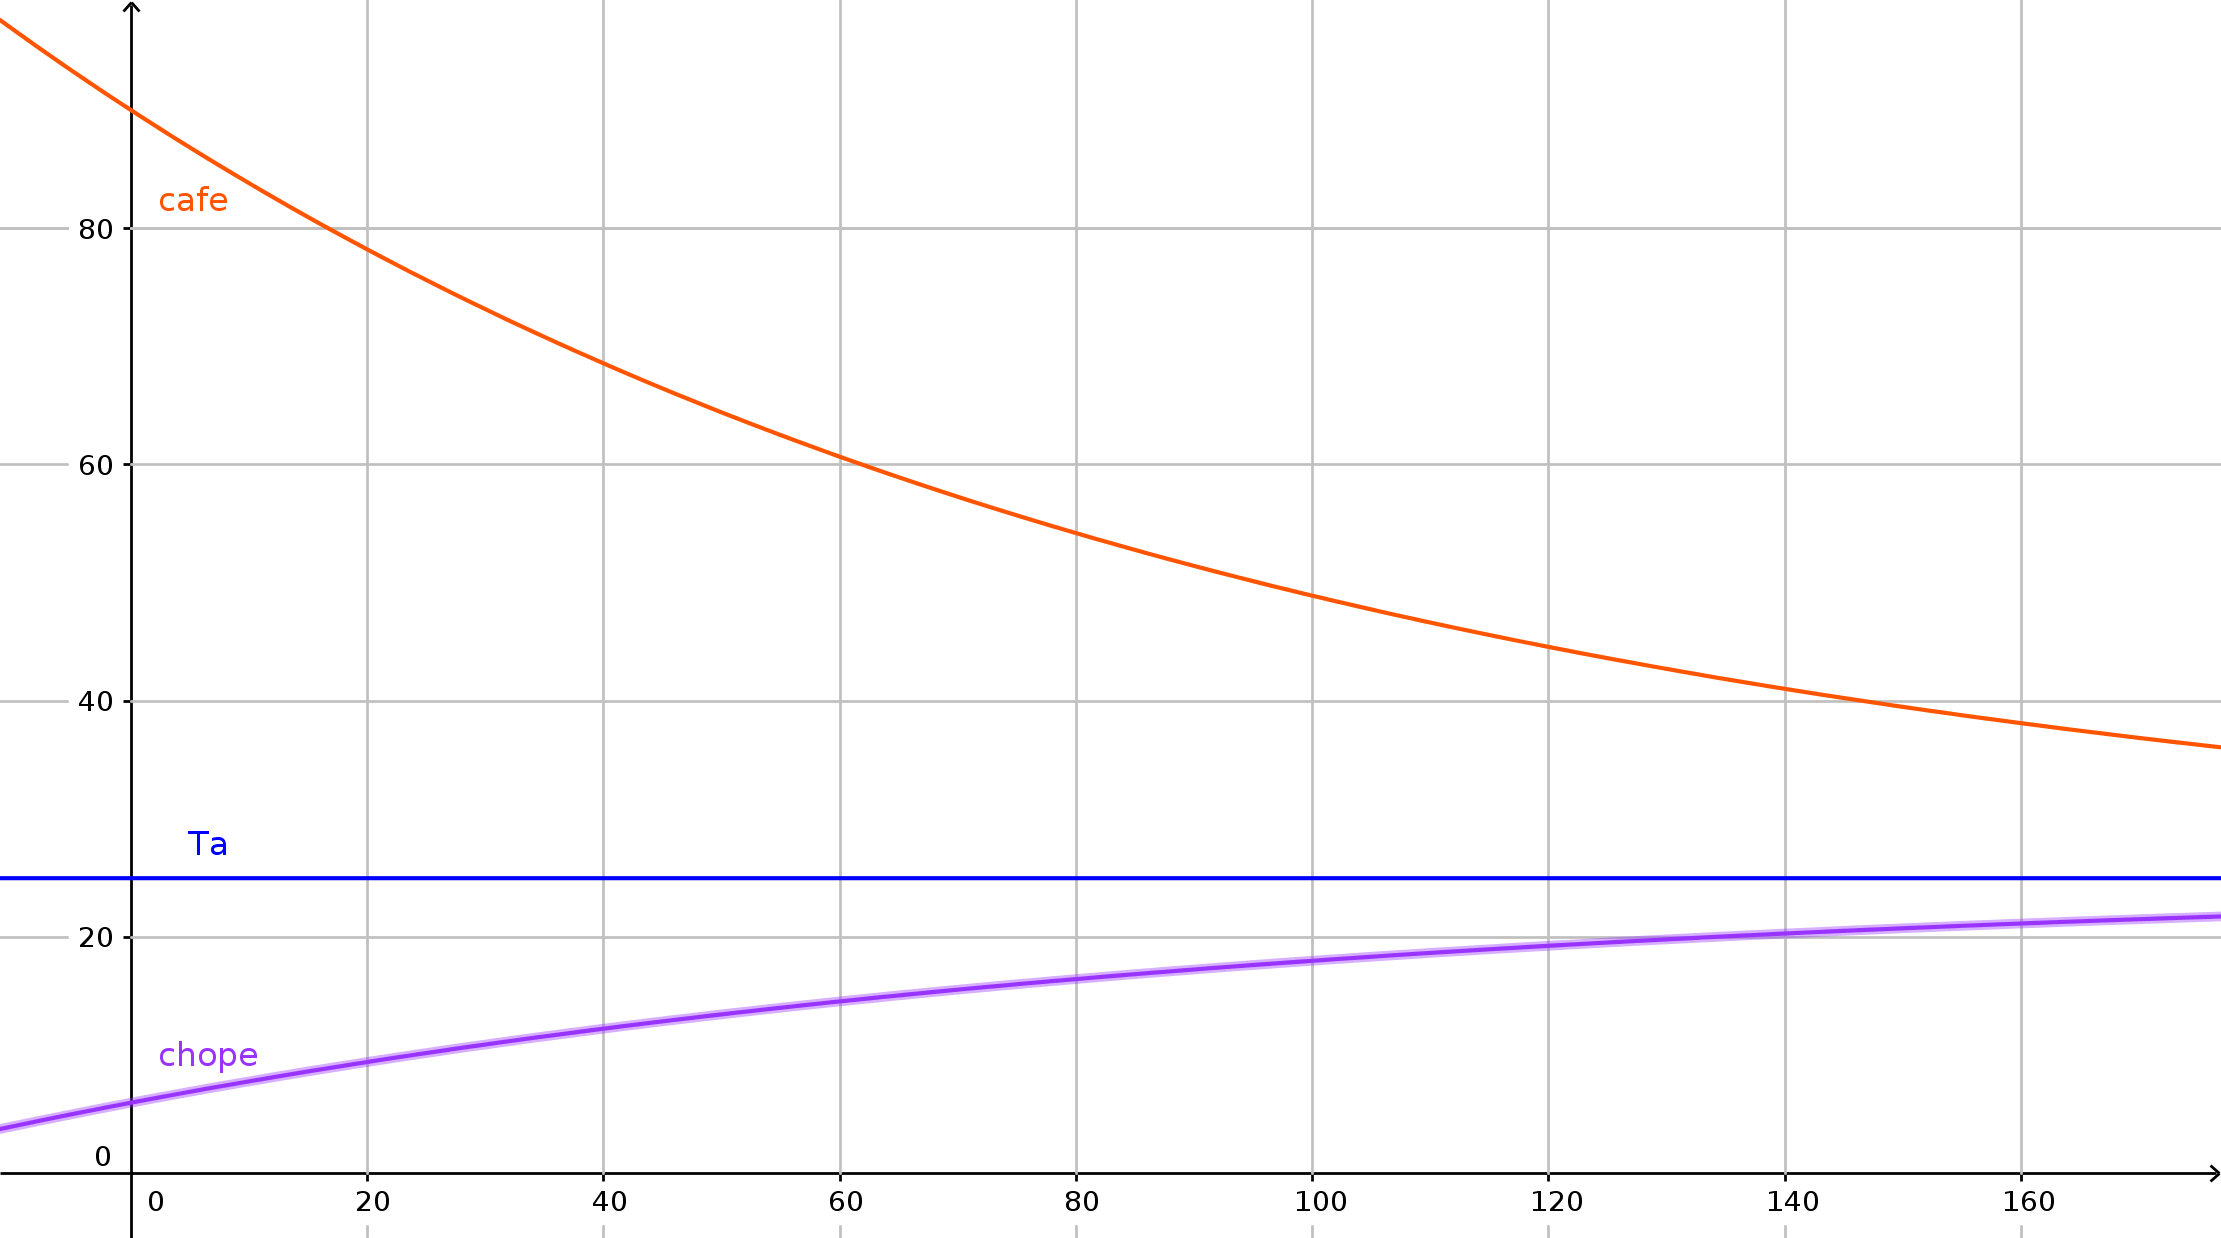
\includegraphics[width=.9\textwidth]{cafe_chope}
\end{center}
\hrulefill

{\bf Desafio:} Qual é o limite dessas duas funções quando
$t\rightarrow \infty$? O que você pode concluir desse resultado?

\subsection{Meia vida: decaimento radioativo}


\end{document}
